\documentclass{standalone}
\usepackage{pgfplots}
\pgfplotsset{compat=1.18}
\usepackage{amsmath}

\begin{document}
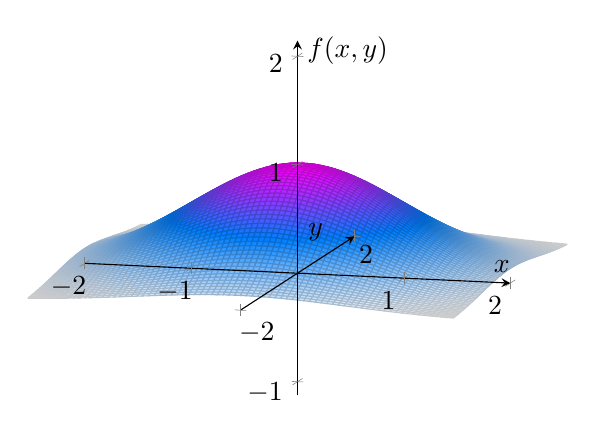
\begin{tikzpicture}
    \begin{axis}[
        xlabel=$x$,
        ylabel=$y$,
        zlabel={$f(x,y)$},
        colormap/cool,
        domain=-2:2,
        domain y=-2:2,
        samples=75,
        samples y=75,
        axis equal,
        axis lines = center,
        axis on top,
        view={15}{10}
    ]
    \addplot3[
        surf,
    ] {exp(-((x^2 + y^2)/2))};
    \end{axis}
\end{tikzpicture}
\end{document}
